In Figure~\ref{fig:overview}, we illustrate a 2D geometry of the proposed vision-correcting display for myopic eyes (top) and hyperopic eyes (bottom). The proposed framework consists of three planes: the light field display plane ($D$-plane), the virtual image plane ($V$-plane), and the eye's pupil plane ($P$-plane). Widths of each plane are denoted as: $w_d$ (for $D$-plane), $w_v$ (for $V$-plane), and $w_p$ (for $P$-plane), and these widths satisfy the following relationship:
\[ w_v =
  \begin{cases}
    (1-\alpha)w_l-\alpha w_p  & \quad \text{for myopia}\\
    (1+\alpha)w_l-\alpha w_p  & \quad \text{for hyperopia}\\
  \end{cases}
\]
where $\alpha$ is the ratio $d_v/d_e$, where $d_v$ and $d_e$ are distances from D-plane to V-plane and P-plane, respectively. 

\begin{figure}[t]
	    \begin{center}
		%\fbox{\rule{0pt}{2in} \rule{0.9\linewidth}{0pt}}
   		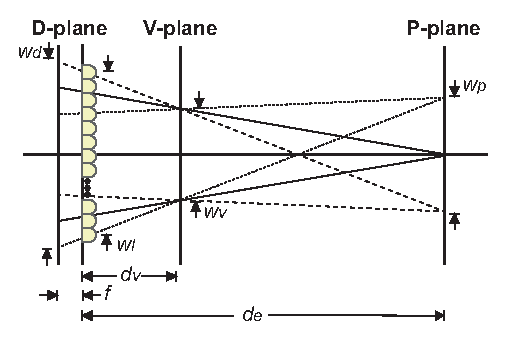
\includegraphics[width=0.95\linewidth]{images/overview_myopic.eps}
	    \end{center}
	    \begin{center}
		%\fbox{\rule{0pt}{2in} \rule{0.9\linewidth}{0pt}}
   		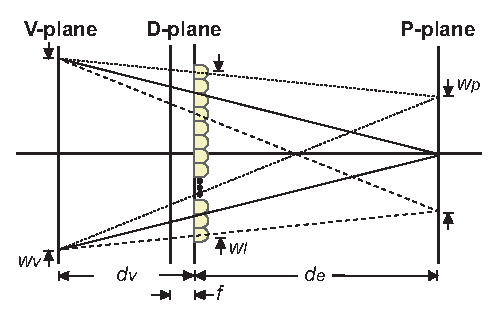
\includegraphics[width=0.95\linewidth]{images/overview_hyperopia.eps}
	\end{center}
	\caption{Geometry of the proposed framework for correcting myopia (top) and hyperopia (bottom). $D$-plane: light field display plane, $V$-plane: the virtual image plane, and $P$-plane: the eye's pupil plane}
\label{fig:overview}
\end{figure}

Following the notion of Zwicker~\etal~\cite{zwicker2006antialiasing}, let us suppose the light field display has angular and spatial sample space as $\Delta v$ and $\Delta t$, respectively. In Figure~\ref{fig:overview}, we explained angular and spatial resolutions of the light field display using microlens (or lenslet) array, which is placed a focal distance $f$ in front of the 2D display. Note that, various types of light field display (\ie, pin-hole array) are adoptable to the proposed system.

Field of view (FOV), which indicates the extent of the observable image through the display, is limited by widths of the virtual image ($w_v$) and the display ($w_d$).
\[ \text{FOV} =
  \begin{cases}
    2\arctan\Big(\min\Big[\frac{w_l}{2d_e}, \frac{w_v}{2(d_e-d_v)}\Big]\Big)  & \quad \text{for myopia}\\
    2\arctan\Big(\min\Big[\frac{w_l}{2d_e}, \frac{w_v}{2(d_e+d_v)}\Big]\Big)  & \quad \text{for hyperopia}\\
  \end{cases}
\]

%\begin{equation}
%\textsc{FOV} = 2\arctan\Big(\min\Big[\frac{w_l}{2d_e}, \frac{w_v}{2(d_v+d_e)}\Big]\Big)
%\end{equation}

%The magnification of the virtual image depends on the distance $d_v$ and the width of display $w_d$.

%\begin{equation}
%M = \frac{w_d}{d_e} \times (d_e-d_v-f)
%\end{equation}

\subsubsection{Spatial and Angular Resolution Requirements}
For light field rendering of 2D object placed at the constant depth, Chai~\etal~\cite{chai00} have shown the maximum spatial resolution for light fields reconstruction of object without aliasing can be determined by the following two factors: the angular resolution and the spatial sampling rate of the virtual image ($\Delta s$). Given an virtual image placed $d_v$ from the display, the maximum spatial spacing can be derived as follows:
\begin{equation}
\Delta t_{\max} = d_v \max( \Delta v, 2\Delta s )/f
\end{equation}
Note that, $\Delta s$ should be bounded by the highest spatial sampling rate of human retinal vision $\Delta u~(\leq \Delta s)$, which is approximately one cycle per arcmin [REF!]. Pamplona~\etal~\cite{pamplona12} has shown the required pixel pitch of displays that matches to the maximum human retinal resolution. As mentioned in Chai~\etal, if we can remove high frequency components of 2D object by applying low-pass filtering, which satisfies $\Delta s > 2\Delta v$, and the equation can be reduced as follows:
\begin{equation}
\Delta t_{\max} = d_v \Delta v/f 
\label{eq:resolutionLimits}
\end{equation}
To satisfy the condition $\Delta s > 2\Delta v$, $w_v$ should be larger than $2fw_d/d_v$ (for the proof, see supplemental materials). According to Zwicker~\etal, light fields can be rendered maximizing the use of spatial resolution of display if it satisfies $|d_v| \leq f\Delta t/\Delta v$. This indicates a virtual image placed farther than $f\Delta t/\Delta v$ will be rendered blurred.

% consider human eye resolution limit (1 arcmin), which gives the min of an object size
% also set limit to the max viewing zone